\documentclass[10pt]{article}
\usepackage[final]{graphicx}
\usepackage{amsfonts}

\topmargin -.5in
\textwidth 6.6in
\textheight 9in
\oddsidemargin 0in
\usepackage{color}
\newcommand{\arvind}[1]{{\color{red}{Arvind: {#1}}}}

\def\ds{\displaystyle}
\def\d{\partial}

\begin{document}

\centerline{\large \bf Fusing surface and satellite-derived PM observations to determine the impact } 

\centerline{\large \bf of international transport on coastal PM$_{2.5}$ concentrations in the western U.S.}


\vspace{.3truein}
\section{The approach}

\subsection{Relationships between AVHRR AOD and surface PM$_{2.5}$}
We noticed that there was a huge difference between the  $4$ sites we identified along the West Coast and the $9$ sites located on Hawaii. The sites on Hawaii are unique because Hawaii is surrounded on water. Thus we decided to build models only for both the sites along the West Coast. We also noticed that there was different relationships between AOD and PM among each site from the Figure \ref{ig3.2.1}. So we analyzed the relation for each site. 

\begin{figure}[!h]
\centering
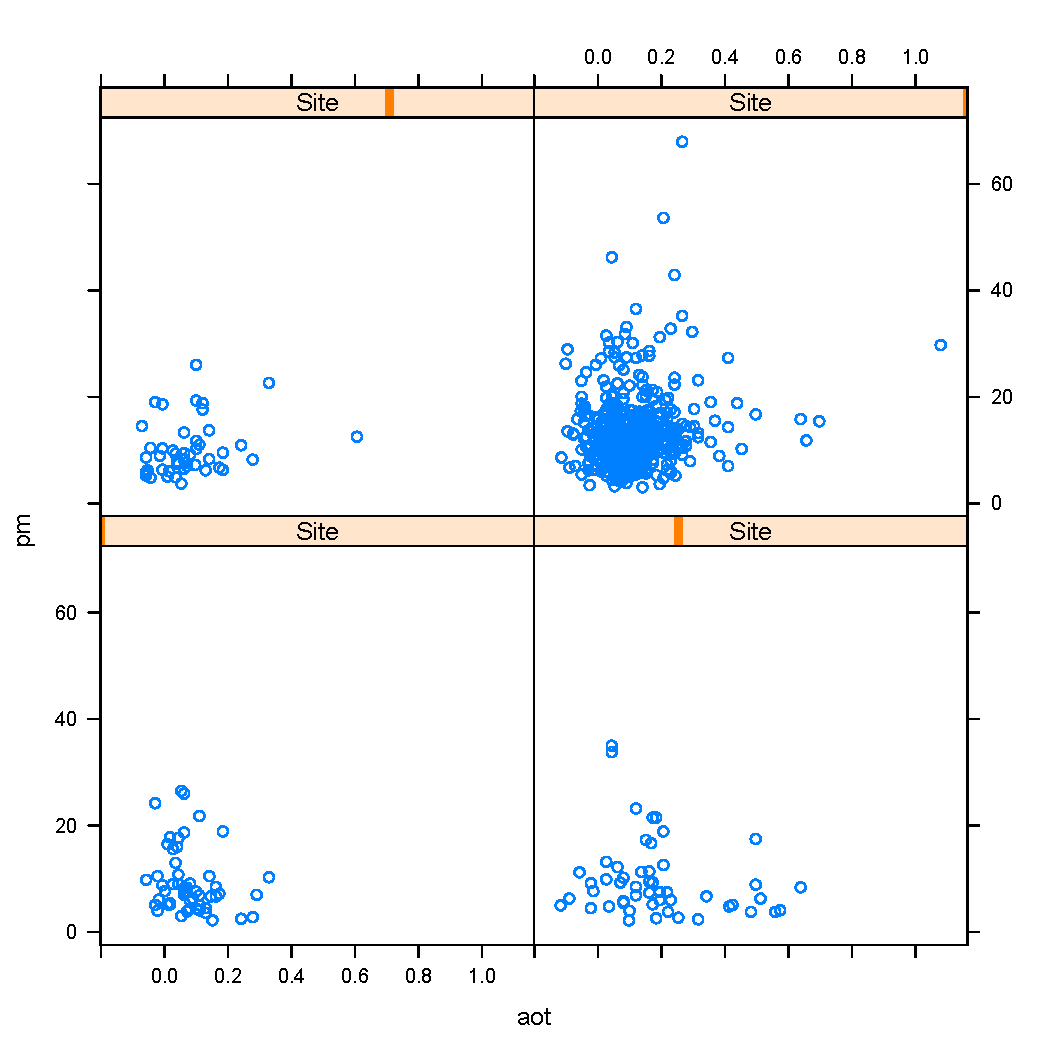
\includegraphics[width = 0.6\linewidth]{3.pdf}
\caption{PM vs. AOD for west coast sites}
\label{fig3.2.1}
\end{figure}


\subsubsection{Only AOD data}
Since there are many meteorological parameters varying from day to day, our statistical model must have the variability of the date. For each location, there are many different geographical properties, so our model must have the variability of sites. Therefore we used mixed effects model to fit this relationship:

$$PM_{ij} = \alpha + \beta\times AOD_{ij} + s_i + d_j+ \epsilon_{ij}, $$

where $PM_{ij}$ is the $PM_{2.5}$ concentration at a spatial site $i$ on a specific day $j$, $\alpha$ is the fixed intercept, $\beta$ is the fixed slope, $AOD_{ij}$ is the AOD value at a spatial site $i$ on a specific day $j$, $s_i\sim N(0, \sigma_s^2)$ is the random intercept of site $i$, $d_j\sim N(0, \sigma_d^2)$ is the random intercept of a specific day $j$, and $\epsilon_{ij}\sim N(0, \sigma^2)$ is the error term at site $i$ on a day $j$.

\subsubsection{AOD data and wind data}
As we have more information about the time-varying parameters, like air temperature, humidity, etc, it is not reasonable to simply treat them as a random variable. 

First, we tried the multivariate linear regression model to fit the relation. Since the result was not good enough, we tried another kind of model, the gam model, which turned out to be a better model to fit the relationship.

\section{Computational Experiments}

\subsection{Experiment 2: PM 25 vs AOT data}
If we only use the AOD data, by using the approach in Section 3, we fitted the mixed effects model as follows.

$$\hat{PM}_{ij} = 10.51 + 3.60\times AOD_{ij} + \hat{s}_i + \hat{d}_j, $$

where $\hat{s}_i\sim N(0, 1.79^2)$ and $\hat{d}_j\sim N(0, 3.04^2)$. 

The correlation between the fitted PM$_{2.5}$ data and the true PM$_{2.5}$ data is 0.802, which we agreed it is not a bad fit. 

If we use both the AOD data and the wind data, we built a multivariate linear regression model. 
The following analysis is about the site (40.80178, -124.1621) since the relation is different for different sites as mentioned in Section 3. For other sites, analysis should be similar. 

$$\hat{PM} = -0.64 - 0.0176\times AOD - 0.11\times WindSpeed + 0.45\times WindDirection + 0.017\times Humidity$$
$$ - 0.16\times AirTemp + Season + Year, $$

where Season and Year are factor variables. $R^2 = 0.758$.

\begin{figure}[ht!]
\centering
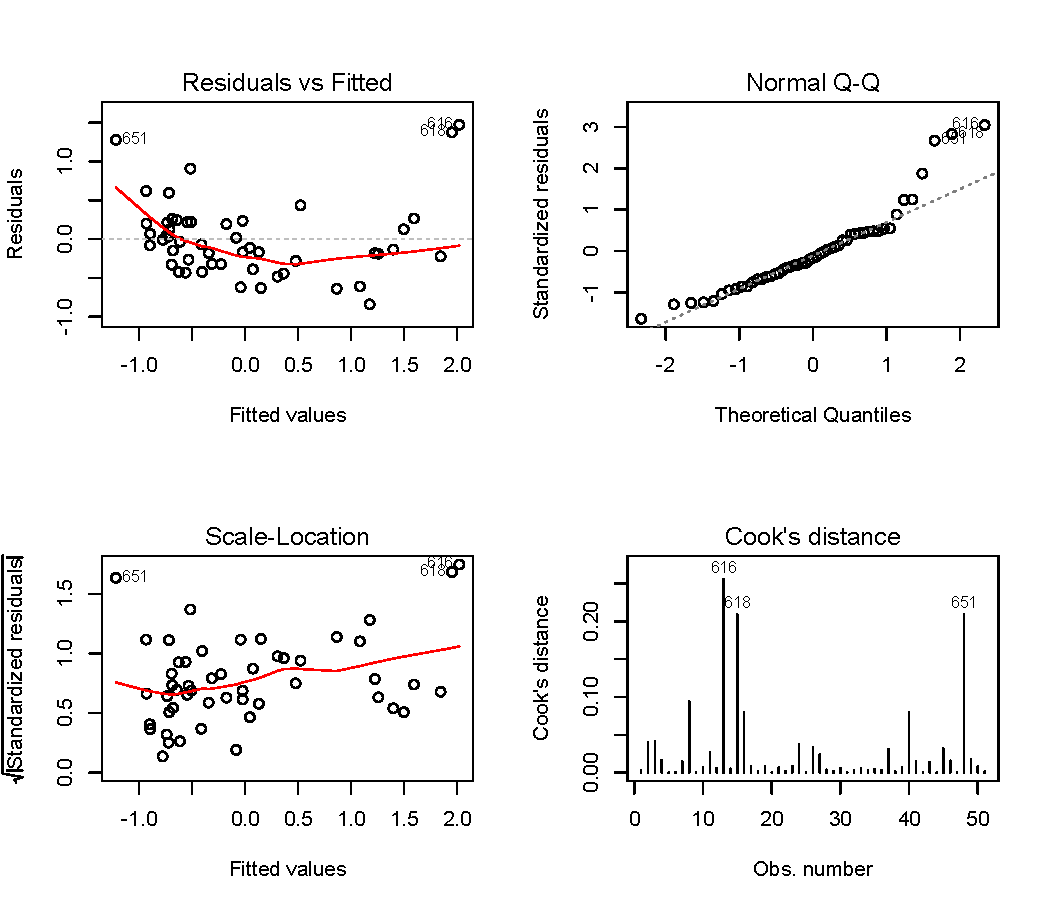
\includegraphics[width = 0.7\linewidth]{residual.pdf}
\caption{Diagnosis 2}
\label{d1}
\end{figure}

We can see from Figure\ref{d1} that there are three outliers. After deleting these outliers, the model became:

$$\hat{PM} = 94.43 + 2.34\times AOD - 1.11\times WindSpeed + 0.033\times WindDirection - 0.068\times Humidity $$
$$- 0.30\times AirTemp + Season + Year, $$

where Season and Year are factor variables. $R^2 = 0.822$.

Then we did the stepwise to choose the best fit, we get the following model:

$$\hat{PM} = 3.42 -1.07\times WindSpeed + 0.036\times WindDirection + Season, $$
where Season is a factor variable. $R^2 = 0.786$.

\begin{figure}[ht!]
\centering
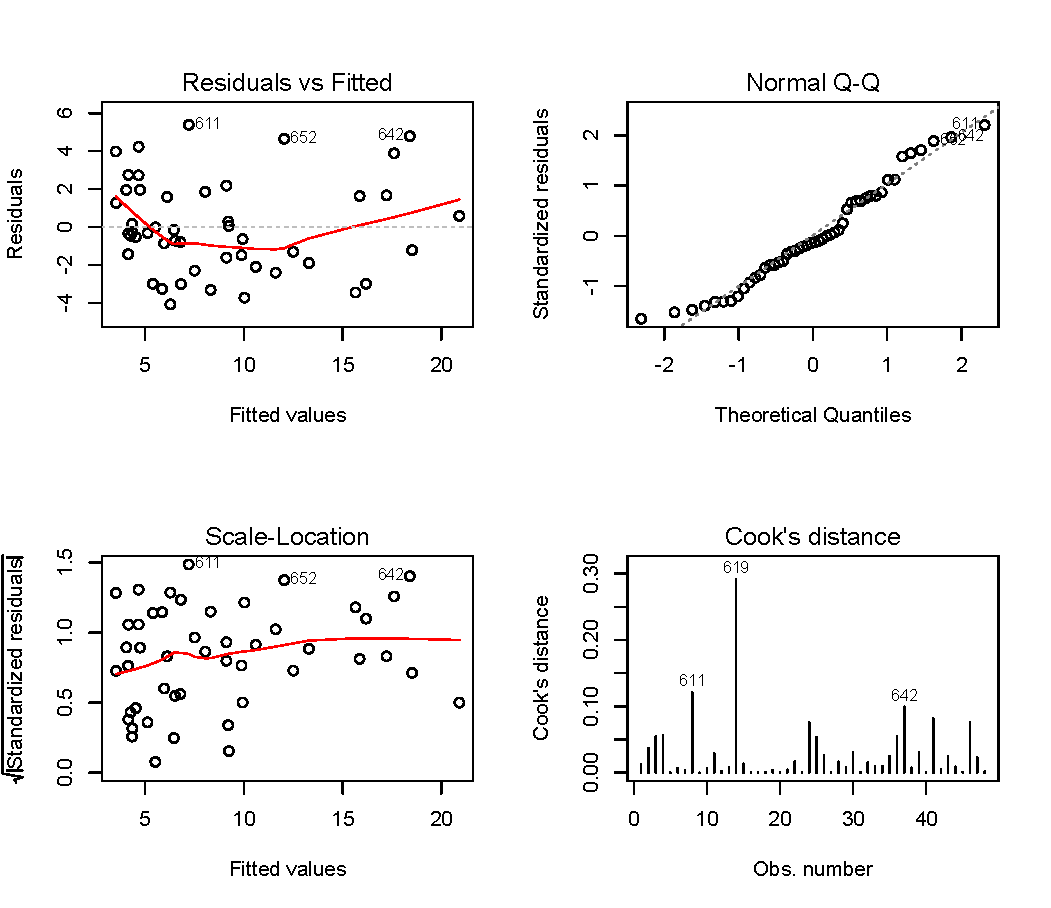
\includegraphics[width = 0.7\linewidth]{residual2.pdf}
\caption{Diagnosis 2}
\label{d2}
\end{figure}

Figure\ref{d2} are the diagnosis plots. Results are better than the previous model. But we can see from those plots that the residuals still have some trend and some cluster, which shows that there must be some violation against the assumptions, like the equal variance assumption for the linear regression model. To figure out if this model is good, we did 5-folder cross validation. The results are as follows:

\begin{figure}[ht!]
\centering
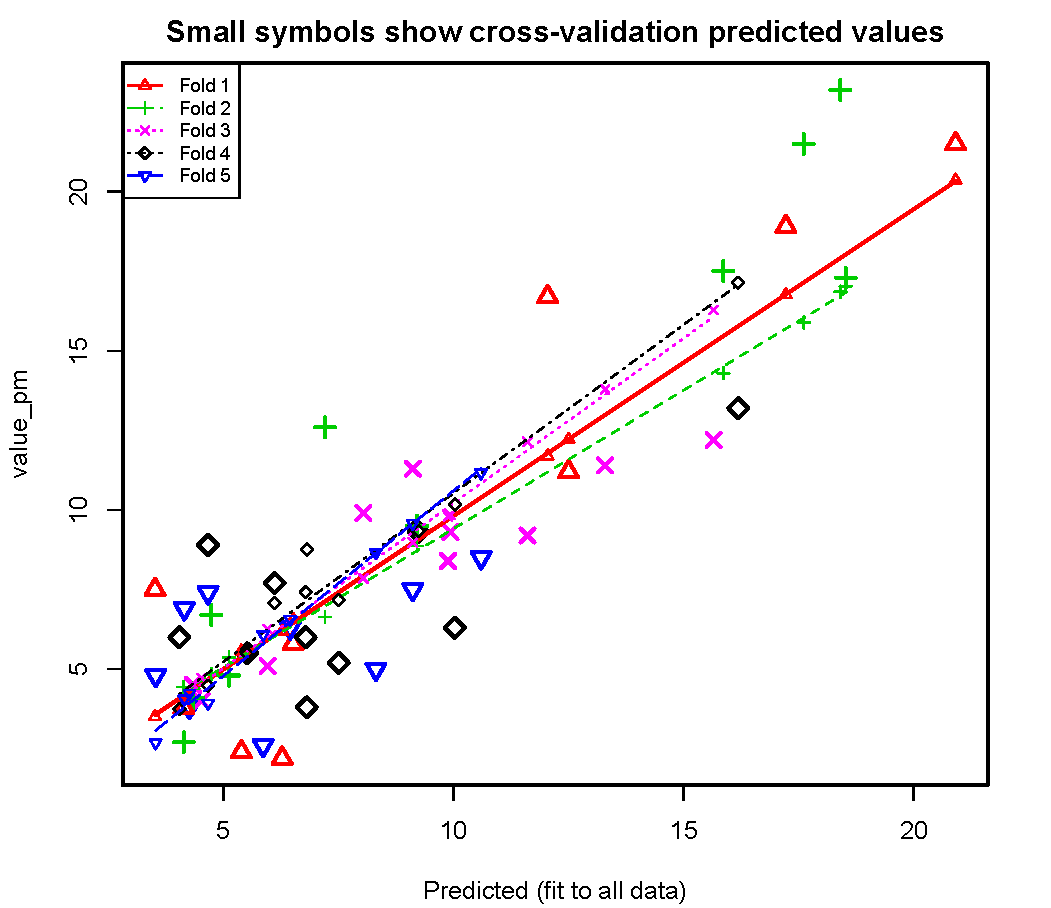
\includegraphics[width = 90mm]{cv_lm.pdf}
\caption{}
%\label{graph5}
\end{figure}

The mean square error is 8.16, which is very high due to the average PM values is 8.75. So we concluded that the multivariate linear regression model is not good.


\end{document}
